\documentclass{article}


\usepackage{siunitx} % Provides the \SI{}{} and \si{} command for typesetting SI units
\usepackage{graphicx} % Required for the inclusion of images
\usepackage{natbib} % Required to change bibliography style to APA
\usepackage{amsmath} % Required for some math elements 
\usepackage{listings}
\usepackage{color}
\setlength\parindent{0pt} % Removes all indentation from paragraphs

\lstset{frame=tb,
  language=Matlab,
  aboveskip=3mm,
  belowskip=3mm,
  showstringspaces=false,
  columns=flexible,
  basicstyle={\small\ttfamily},
  numbers=none,
  numberstyle=\tiny\color{gray},
  keywordstyle=\color{blue},
  commentstyle=\color{dkgreen},
  stringstyle=\color{mauve},
  breaklines=true,
  breakatwhitespace=true,
  tabsize=3
\renewcommand{\labelenumi}{\alph{enumi}.} % Make numbering in the enumerate environment by letter rather than number (e.g. section 6)


\title{Lab 1 \\ Manipulating Sinusoids with Matlab} % Title

\author{Aneesh Malhotra \\ G00844135} % Author name

\date{\today} % Date for the report

\begin{document}

\maketitle % Insert the title, author and date


% If you wish to include an abstract, uncomment the lines below
% \begin{abstract}
% Abstract text
% \end{abstract}

%----------------------------------------------------------------------------------------
%	SECTION 1
%----------------------------------------------------------------------------------------

\section{Introduction}

The objective of this lab was to gain comfort plotting and analyzing sinusoids in Matlab. Initially we created two sinusoids and plotted them, their sum, and their product. We then analyzed the Amplitude and phase of the sum of them using Matlab, and phasor addition. Finally, we created a harmonic function that adds sinusoids whose frequencies are multiples of a given fundamental frequency $f_0$ 


% If you have more than one objective, uncomment the below:
%\begin{description}
%\item[First Objective] \hfill \\
%Objective 1 text
%\item[Second Objective] \hfill \\
%Objective 2 text
%\end{description}

%----------------------------------------------------------------------------------------
%	SECTION 2
%----------------------------------------------------------------------------------------

\section{Main Body}

\subsection{Plotting Sinusoids}

We began by plotting two sinusoids given by 

$$x_1(t) = A_1cos( 2\pi (440)(t- t_{m1}))$$
$$x_1(t) = A_2cos( 2\pi (440)(t- t_{m2}))$$

where $A_2 = 42$ and $A_1 = 0.8 A_2$. The time shifts were given by $ t_{m1} = ?(37.2/8)T$ and $t_{m2} = (41.3/23)T$, where $T = \frac{1}{440}$. We also defined the following:
\begin{align*} 
x_3(t) &= x_1(t) + x_2(t) \\
x_4(t) &= x_1(t) x_2(t) 
\end{align*}
The following plot was obtained

\begin{figure}[t!]
\begin{center}
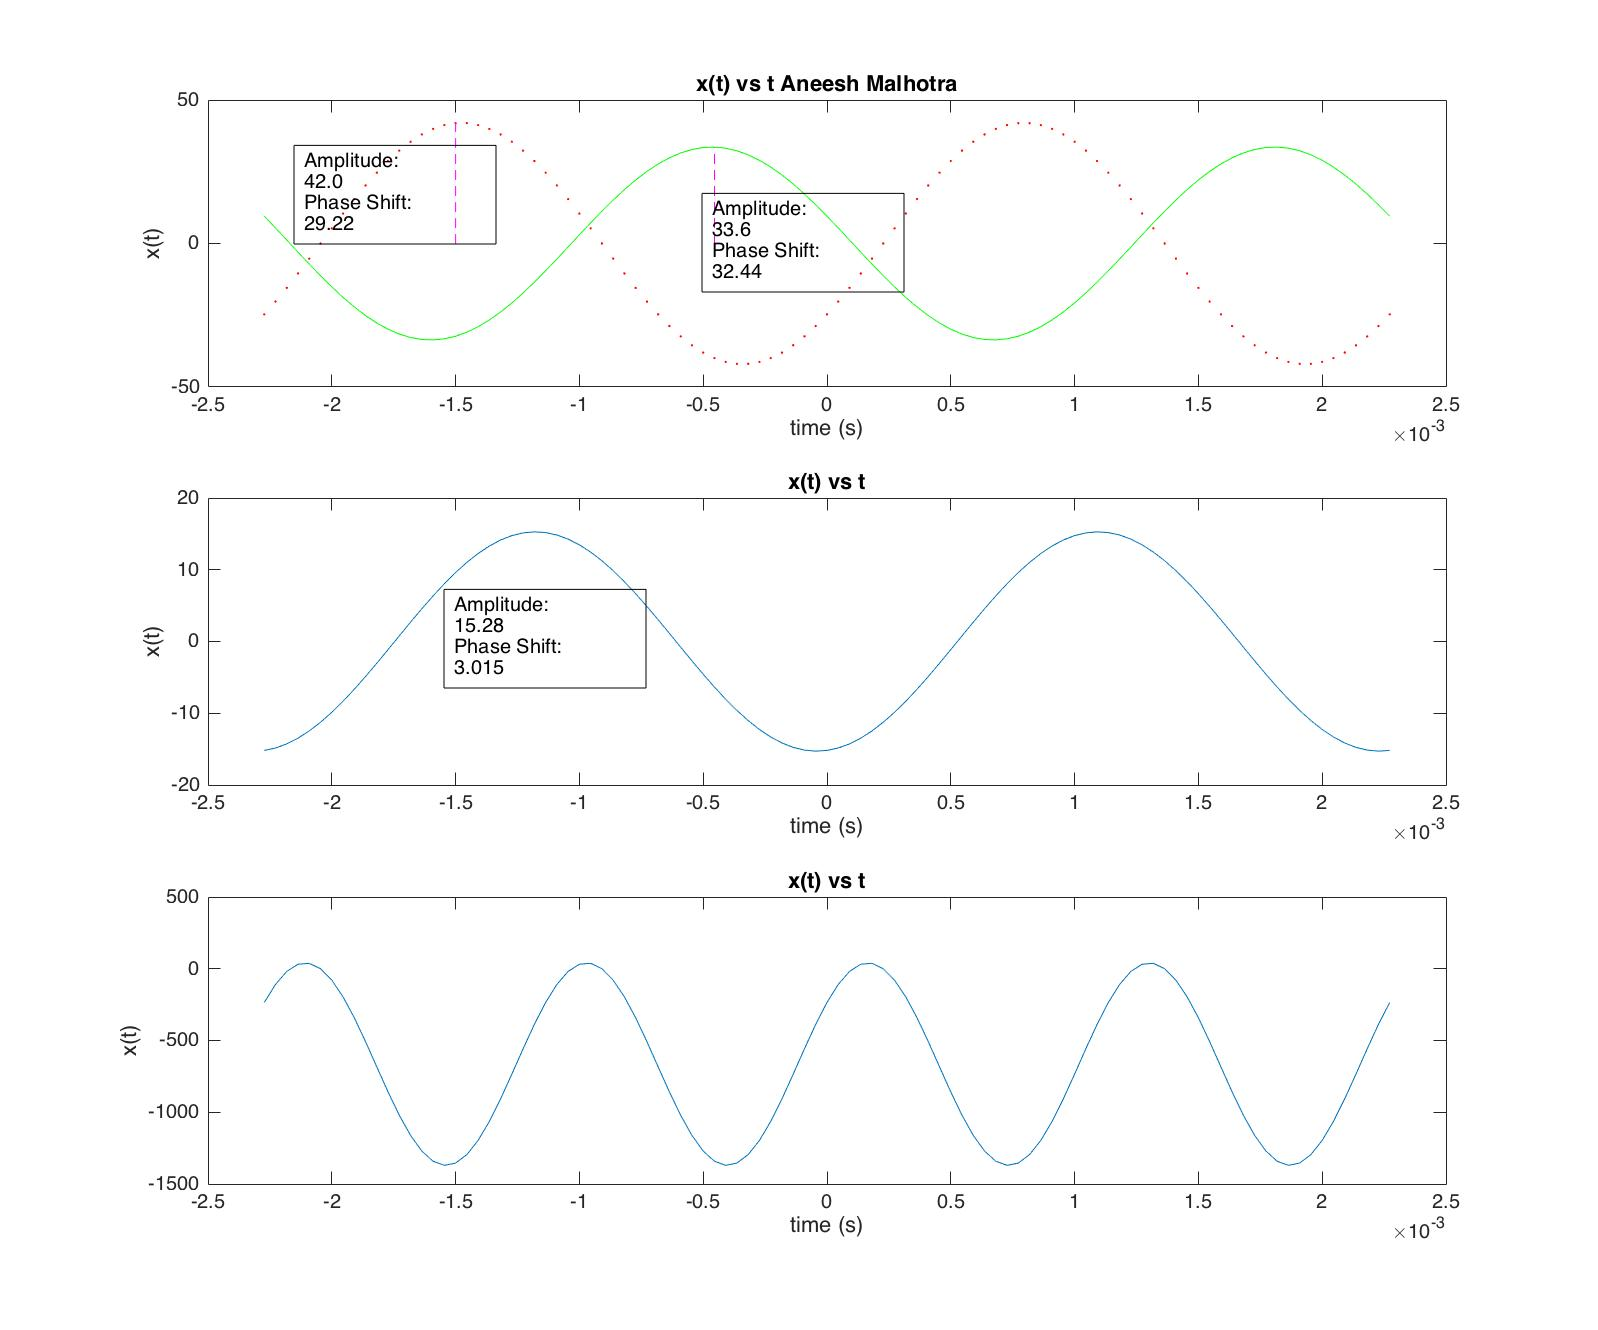
\includegraphics[scale = 0.25]{figure1_part3.jpg}
\caption{Plots of $x_1(t), x_2(t), x_3(t),x_4(t)$ containing approximations of phase and amplitude. Plots $x_1$ and $x_2$ are in the top subfigure, followed by $x_3$ and $x_4$ respectively.}
\end{center}
\end{figure}

By taking the maximum value of $x_3$ in Matlab we approximated the amplitude and phase shift $x_3$. The amplitude was approximately 15.28 and the phase shift was .0068. 

\subsection{Theoretical Calculation of Phase and Amplitude}

We can represent signals $x_1(t)$ and $x_2(t)$ as the real parts of complex exponentials. Therefore, we can represent $x_i(t)$ as the real part of $X_i e ^{j 2 \pi 440}$ where X_i = $A_i e^{j \phi_i}$.
Therefore $$x_1(t) + x_2(t) = \Re\{A_1 e^{j \phi_1} e^{j 2 \pi 440} + A_2 e^{j \phi_2} e^{j 2 \pi 440}\}$$ If we factor out the $e^{j 2 \pi 440}$, we can simply do the addition of the phasors to find the new phasor. Using Matlab, we added the two phasors and found that $|x_3(t)| \approx 15.28145$ and the phase shift was approximately $-3.015$. Phasor addition yielded a phase shift of -3.0267 and a magnitude of 15.28145. These values are consistent with the values obtained using the graph and vector values. 

\subsection {Harmonics}

In this section we created a function that adds sinusoids that are harmonically related. The function takes in values of amplitudes, phases, maximum time, sample period, and fundamental frequency and returns back a sum of sinusoids in the form $$ r(t) = \sum_{n=0} ^N C_n cos(n\omega _0 t + \theta _n).$$ The following plots were obtained for each case, 

\begin{figure}[!htb]
    \centering
    \begin{minipage}{.5\textwidth}
        \centering
        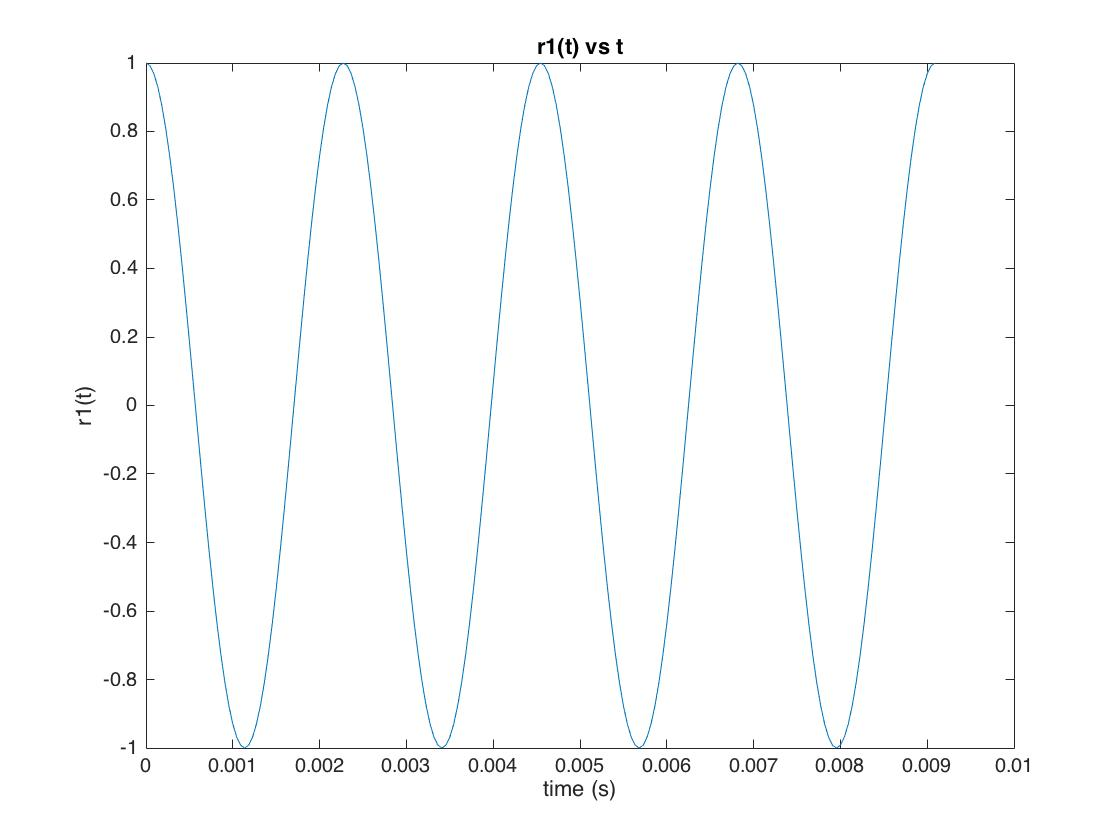
\includegraphics[width=0.8\linewidth, height=0.2\textheight]{figure2_part3.jpg}

        \label{fig:prob1_6_2}
    \end{minipage}%
    \begin{minipage}{0.5\textwidth}
        \centering
        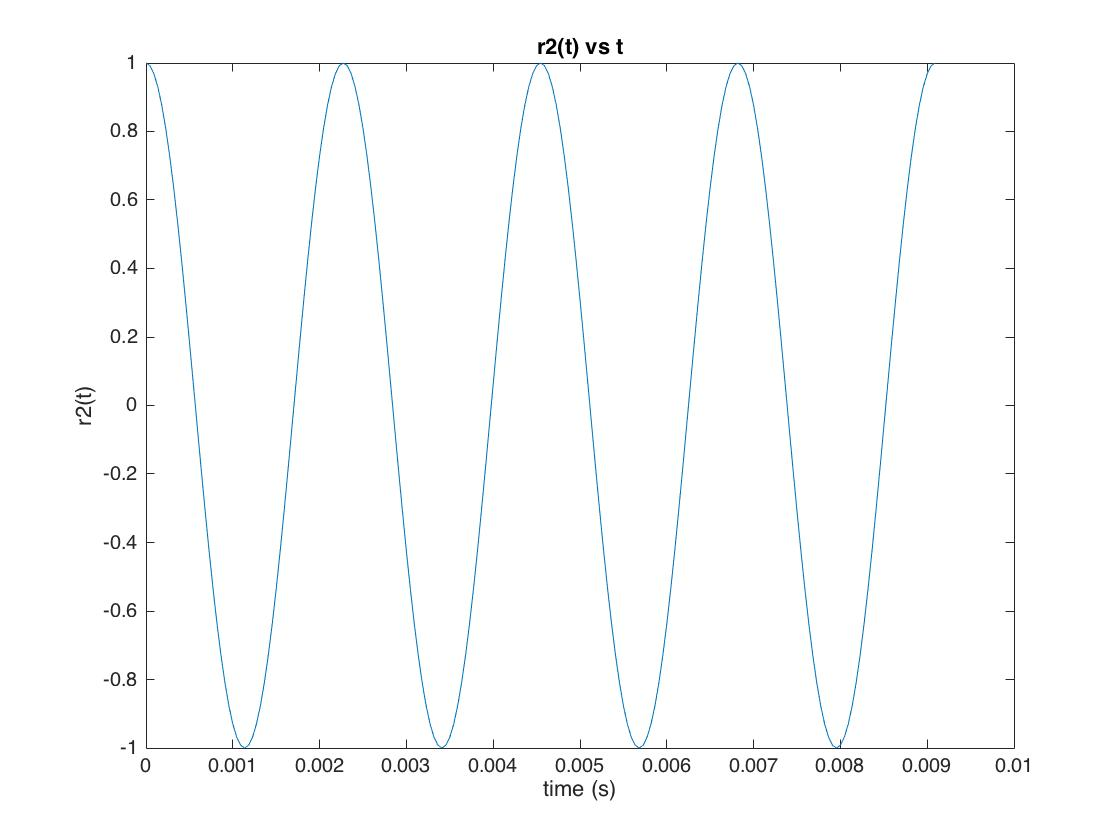
\includegraphics[width=0.8\linewidth, height=0.2\textheight]{figure3_part3.jpg}

        \label{fig:prob1_6_1}
    \end{minipage}
    \caption{Plots of $r_1(t)$ and $r_2(t)$ with the following paramters: $f_0 = 440$, $C_n = [0,1]$, $\theta _n = [0, 0]$ Both had a sample period of 50$}.
\end{figure}

The sounds produced by $r_1$ and $r_2$ were identical and is characterized by a short, medium pitched ring. Upon adding a phase shift, however, we obtain the following plot:

\begin{figure}
\centering
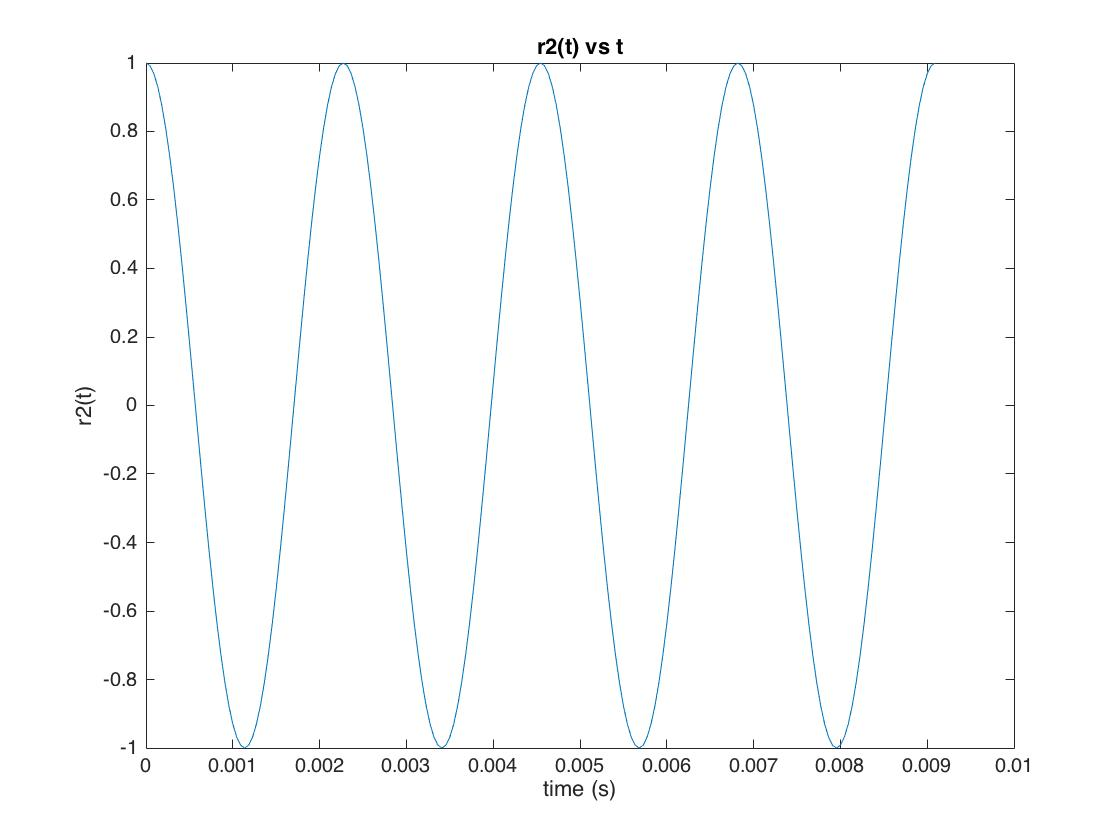
\includegraphics[scale = 0.2] {figure3_part3.jpg}
\caption{The plot of $r_3$ is the same as $r_2$ except with a phase shift}. 
\end{figure}

The phase shift in $r_3$ causes the graph of $r_3$ to look slightly different, although the sound is exactly the same. 



%----------------------------------------------------------------------------------------
%	SECTION 4
%----------------------------------------------------------------------------------------

\section{Conclusion}
In this lab we began by plotting sinusoids. We found that when two sinusoids have the same frequency, the amplitude and phase shift can be found easily by adding the phasors of their corresponding complex exponentials. We saw this when the phase shift and amplitude calculated from the $x_3$ vector were very similar to those calculated by adding phasors. Additionally we looked into the addition of harmonically related sinusoids. By simply adding a phase shift  to one of these signals, we found no noticeable difference in sound. This is because the phase of a signal is not noticeable to the human ear. Therefore, chords played in sync sound the same as they would if they were arpeggiated. 

\section{Appendix}

\subsection{Code to Obtain Plots}
\lstinputlisting{Lab1.m}
\subsection{Harmonic Function}
\lstinputlisting{harmonics.m}
\subsection{Matlab Diary for Calculating Phase}
\lstinputlisting{a.txt}

%----------------------------------------------------------------------------------------
%	BIBLIOGRAPHY
%----------------------------------------------------------------------------------------
\section{References}

Lathi, B. P. Linear Systems and Signals. New York: Oxford UP, 2005. Print.

\end{document}